% Baseline implementation progress report. Compile with: pdflatex main.tex (twice)
\documentclass[conference]{IEEEtran}

\usepackage[T1]{fontenc}
\usepackage{microtype}
\usepackage{booktabs}
\usepackage{graphicx}
\usepackage{tikz}
\usepackage{pgfplots}
\usetikzlibrary{arrows.meta,positioning,shapes.geometric}
\pgfplotsset{compat=1.18}
\usepackage[hidelinks]{hyperref}

\title{Stage 1 Baseline Implementation Report: Attention-Based Instrument Concept Learning for an Explainable Music Genre Classification Framework}
\author{\IEEEauthorblockN{Author Name}\IEEEauthorblockA{Department / University\\City, Country\\author.email@university.edu}}

\begin{document}
\maketitle

\begin{abstract}
This report documents the current baseline implementation of a larger proposed explainable, concept-guided music genre classification framework. The implemented component is Stage~1, instrument concept learning; rhythm, timbre, harmony, concept fusion, and genre classification have not yet been implemented. The baseline treats each song as a bag of precomputed 15-second log-Mel spectrogram windows. A shared convolutional encoder produces a window representation, a learned instrument projection produces 64-dimensional window embeddings, and masked attention-based multiple-instance learning aggregates variable-length songs into a 64-dimensional instrument concept embedding. A multi-label instrument classifier supervises this song-level embedding using binary cross-entropy with logits. On the supplied 40-epoch training history, validation loss decreased from 0.4290 to 0.3631, macro F1 increased from 0.1236 to 0.3104, micro F1 from 0.2699 to 0.5399, and macro mean average precision reached 0.4501 at epoch 37. These results provide measured evidence that the baseline learns useful song-level instrument information, while remaining insufficient to establish end-to-end genre-classification performance.
\end{abstract}

\begin{IEEEkeywords}
music information retrieval, instrument recognition, concept learning, multiple-instance learning, attention pooling, multi-label classification
\end{IEEEkeywords}

\section{Introduction}
Music genre is influenced by several interacting musical properties rather than a single acoustic cue. The broader research direction of this project is an explainable genre classifier that organizes such evidence into learned concepts. The intended progression is instrument concepts, followed by rhythm, timbre, and harmony concepts; their learned song embeddings would then be fused for multi-label genre prediction.

This report concerns only the first completed step. Its purpose is to record the implemented Stage~1 baseline, its experimental behavior, and the technical issues encountered. It does not claim that the complete progressive architecture or a genre classifier has been evaluated. In particular, the observed instrument metrics should be interpreted as feasibility evidence for concept learning, not as a final assessment of the proposed research framework.

\section{Related Work}
Instrument recognition from time--frequency audio representations is commonly approached using convolutional neural networks (CNNs), while music recordings often require multi-label supervision because multiple instrument families can co-occur. Multiple-instance learning (MIL) is appropriate when a song has a recording-level label but the relevant short segments are not annotated. Attention-based MIL provides a learned, differentiable weighting of instances and is therefore useful for forming song-level representations from variable-length sets of windows~\cite{ilse2018attention}.

The baseline combines these established ideas: log-Mel windows are encoded by a CNN, and attention pooling learns the song-level aggregation. The architectural decision to export an intermediate concept embedding is motivated by the future concept-guided framework rather than a claim of a new instrument-recognition method. Standard CNN and audio-representation background may be cited with sources appropriate to the final dissertation or paper~\cite{hershey2017cnn,choi2017transfer}.

\section{Proposed Research Framework and Current Scope}
The proposed full framework is shown in Fig.~\ref{fig:roadmap}. Only the shaded Stage~1 box has been implemented and evaluated in the materials supplied for this report. Stages~2--4, fusion, and genre prediction are planned extensions.

\begin{figure*}[t]
\centering
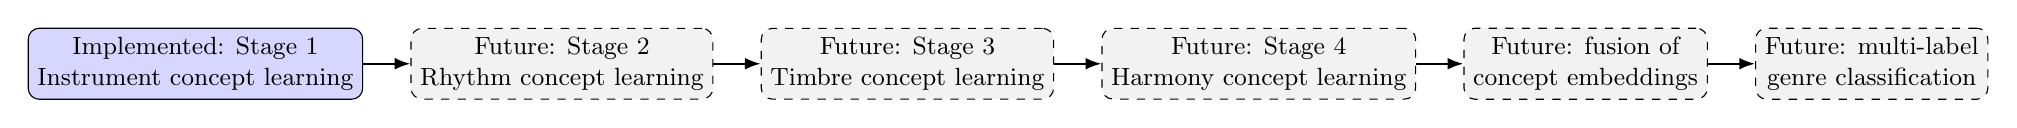
\begin{tikzpicture}[node distance=5mm and 6mm, every node/.style={font=\small}, box/.style={draw, rounded corners, minimum height=8mm, align=center, fill=white}, future/.style={box, dashed, fill=gray!10}, arrow/.style={-{Latex[length=2mm]}, thick}]
\node[box, fill=blue!16] (s1) {Implemented: Stage 1\\Instrument concept learning};
\node[future, right=of s1] (s2) {Future: Stage 2\\Rhythm concept learning};
\node[future, right=of s2] (s3) {Future: Stage 3\\Timbre concept learning};
\node[future, right=of s3] (s4) {Future: Stage 4\\Harmony concept learning};
\node[future, right=of s4] (fusion) {Future: fusion of\\concept embeddings};
\node[future, right=of fusion] (genre) {Future: multi-label\\genre classification};
\draw[arrow] (s1)--(s2); \draw[arrow] (s2)--(s3); \draw[arrow] (s3)--(s4); \draw[arrow] (s4)--(fusion); \draw[arrow] (fusion)--(genre);
\end{tikzpicture}
\caption{Research roadmap. Blue denotes the implemented and evaluated baseline; dashed boxes are proposed future work.}
\label{fig:roadmap}
\end{figure*}

\section{Implemented Baseline Methodology}
\subsection{Input preparation}
The supplied notebook consumes a manifest of available songs and precomputed, per-song stacked NumPy arrays. Each array has shape $(W,128,469)$, where $W$ is the variable number of windows in a song, 128 is the number of Mel bands, and 469 is the number of Mel frames. The original pipeline represents audio as non-overlapping 15-second windows (15-second window and hop sizes) and limits a song to 240 seconds. The training notebook intentionally does not rescan or concatenate individual windows; it loads the complete stacked log-Mel array for each song. Details not recorded in the notebook, such as sample rate, FFT size, and Mel-frequency bounds, are not specified here.

During batching, the variable window dimension is zero-padded and a Boolean mask identifies valid windows. The mask is used by attention pooling so that padding cannot affect the song embedding. The manifest supplies the instrument targets; ten label columns were inferred: percussion, guitar, bass family, keyboard, strings family, brass family, woodwinds, electronic, orchestra, and voice.

\subsection{Architecture}
Fig.~\ref{fig:baseline} follows the executed model rather than an intended extension. Each window first passes through a shared CNN comprising three $3\times3$ convolutional blocks with 32, 64, and 128 channels, batch normalization, ReLU activations, and pooling. Adaptive average pooling followed by a linear layer and ReLU gives a 512-dimensional window feature. The \texttt{InstrumentHead} then maps it to a 64-dimensional window embedding using a linear layer and ReLU.

For a song with embeddings $z_i\in\mathbb{R}^{64}$, a small attention network computes $s_i=\mathbf{w}_2^T\tanh(\mathbf{W}_1z_i)$, where the hidden size is 32. With the padded positions masked, $a_i=\mathrm{softmax}(s_i)$ and the song embedding is $z=\sum_i a_i z_i$. A final linear classifier maps $z$ to ten instrument logits. Thus, the exported 64-dimensional attention-pooled vector is the current instrument concept embedding.

\begin{figure}[t]
\centering
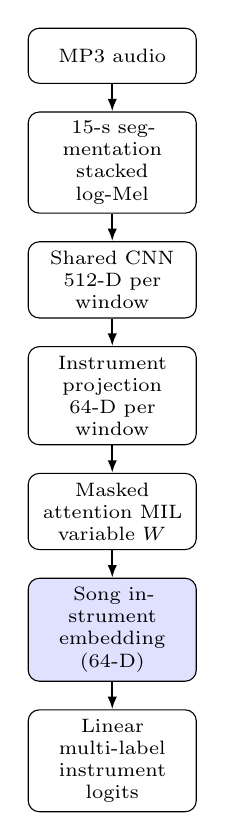
\begin{tikzpicture}[node distance=3.5mm, every node/.style={font=\scriptsize}, box/.style={draw, rounded corners, align=center, minimum height=7mm, text width=19mm}, arrow/.style={-{Latex[length=1.6mm]}, thick}]
\node[box] (audio) {MP3 audio};
\node[box, below=of audio] (mel) {15-s segmentation\\stacked log-Mel};
\node[box, below=of mel] (cnn) {Shared CNN\\512-D per window};
\node[box, below=of cnn] (head) {Instrument projection\\64-D per window};
\node[box, below=of head] (attn) {Masked attention MIL\\variable $W$};
\node[box, below=of attn, fill=blue!12] (embed) {Song instrument\\embedding (64-D)};
\node[box, below=of embed] (class) {Linear multi-label\\instrument logits};
\draw[arrow] (audio)--(mel); \draw[arrow] (mel)--(cnn); \draw[arrow] (cnn)--(head); \draw[arrow] (head)--(attn); \draw[arrow] (attn)--(embed); \draw[arrow] (embed)--(class);
\end{tikzpicture}
\caption{Implemented Stage~1 baseline. Attention pools the projected window embeddings; the classifier supervises the resulting song embedding.}
\label{fig:baseline}
\end{figure}

\subsection{Optimization and reproducibility}
The model uses \texttt{BCEWithLogitsLoss}, consistent with multi-label instrument targets. Optimization uses AdamW with learning rate $10^{-4}$ and weight decay $10^{-4}$. Gradients are clipped to a norm of 1.0. The notebook enables CUDA automatic mixed precision when a GPU is available and uses a \texttt{ReduceLROnPlateau} scheduler (factor 0.5, patience 2) driven by validation loss. Predictions are thresholded at 0.5 for F1. The notebook records parameters and per-epoch metrics with MLflow, saves best and last checkpoints, and exports the attention-pooled embeddings to Parquet.

\section{Experimental Setup}
The notebook snapshot is explicitly configured in development mode. It samples 5,000 available songs with seed 42, caches the selected stacked Mel arrays on Colab local SSD, uses batch size 16 and two loader workers, and splits validation at 15\% when a usable manifest split is unavailable. The code uses existing train/validation/test-like manifest labels if both training and validation partitions are present. Table~\ref{tab:config} records only settings visible in the source artifacts.

\begin{table}[t]
\caption{Recorded baseline configuration.}
\label{tab:config}
\centering\footnotesize
\begin{tabular}{ll}
\toprule
Item & Value \\
\midrule
Development sample & 5,000 songs \\
Instrument classes & 10 \\
Window / hop & 15 s / 15 s \\
Maximum duration & 240 s \\
Input per window & $1\times128\times469$ \\
Batch size / workers & 16 / 2 \\
Optimizer & AdamW ($10^{-4}$, $10^{-4}$ decay) \\
Validation fraction & 0.15 (fallback) \\
F1 threshold & 0.5 \\
Random seeds & 42 \\
\bottomrule
\end{tabular}
\end{table}

\textit{Run provenance.} The notebook snapshot displays an override of 20 epochs, whereas the supplied training-history CSV contains epochs 1--40. This report treats the CSV as the source of the reported 40-epoch metrics, but does not infer why its epoch count differs from the snapshot. All remaining configuration statements above come directly from the notebook.

\section{Results}
The reported curves are generated directly from \texttt{training\_history\_40\_epochs.csv}, included with this project. Validation computes macro mean average precision (mAP) from probabilities and macro/micro F1 from 0.5-thresholded probabilities. Table~\ref{tab:results} summarizes the initial, intermediate, best, and final observations.

\begin{figure}[t]
\centering
\begin{tikzpicture}
\begin{axis}[width=\columnwidth,height=4.5cm,xlabel={Epoch},ylabel={Loss},grid=major,legend style={font=\scriptsize,at={(0.98,0.98)},anchor=north east},legend cell align=left]
\addplot[blue,thick] table[x=epoch,y=train_loss,col sep=comma]{training_history_40_epochs.csv};
\addlegendentry{Training}
\addplot[red,thick] table[x=epoch,y=val_loss,col sep=comma]{training_history_40_epochs.csv};
\addlegendentry{Validation}
\end{axis}
\end{tikzpicture}
\caption{Training and validation loss across the supplied 40-epoch history.}
\label{fig:loss}
\end{figure}

\begin{figure}[t]
\centering
\begin{tikzpicture}
\begin{axis}[width=\columnwidth,height=4.5cm,xlabel={Epoch},ylabel={Score},ymin=0,ymax=0.60,grid=major,legend style={font=\scriptsize,at={(0.02,0.98)},anchor=north west},legend cell align=left]
\addplot[blue,thick] table[x=epoch,y=macro_f1,col sep=comma]{training_history_40_epochs.csv}; \addlegendentry{Macro F1}
\addplot[red,thick] table[x=epoch,y=micro_f1,col sep=comma]{training_history_40_epochs.csv}; \addlegendentry{Micro F1}
\addplot[black,dashed,thick] table[x=epoch,y=macro_map,col sep=comma]{training_history_40_epochs.csv}; \addlegendentry{Macro mAP}
\end{axis}
\end{tikzpicture}
\caption{Validation macro F1, micro F1, and macro mAP.}
\label{fig:metrics}
\end{figure}

\begin{table}[t]
\caption{Validation progression from the supplied history. Best values are selected per metric.}
\label{tab:results}
\centering\scriptsize
\begin{tabular}{crrrrr}
\toprule
Epoch & Train loss & Val. loss & Macro F1 & Micro F1 & Macro mAP \\
\midrule
1  & .4768 & .4290 & .1236 & .2699 & .2997 \\
10 & .3907 & .3932 & .2141 & .4304 & .3878 \\
20 & .3739 & .3745 & .2638 & .4929 & .4334 \\
30 & .3665 & .3858 & .2309 & .4483 & .4430 \\
37 & .3626 & .3646 & .2928 & .5215 & \textbf{.4501} \\
40 & \textbf{.3617} & \textbf{.3631} & \textbf{.3104} & \textbf{.5399} & .4475 \\
\bottomrule
\end{tabular}
\end{table}

\subsection{Loss analysis and convergence}
Fig.~\ref{fig:loss} shows a substantial early reduction in both losses. Training loss falls from 0.4768 to 0.3617 and validation loss from 0.4290 to 0.3631. Although validation loss is not monotonic---for example, it is 0.3858 at epoch 30---it ultimately reaches its lowest logged value at epoch 40. The narrow final difference between training and validation loss (approximately 0.0014) does not indicate a large loss-based generalization gap in this run. However, a single development-mode history does not establish robustness across resamples or full-scale training.

\subsection{F1 and mAP analysis}
Macro F1 improves by 0.1868 from epoch 1 to epoch 40, while micro F1 improves by 0.2700. The lower macro than micro F1 is consistent with unequal label difficulty or prevalence, but the supplied history alone does not identify the responsible classes. Macro mAP rises from 0.2997 to 0.4475 and peaks marginally higher at 0.4501 in epoch 37. Together, the sustained improvement in ranking quality (mAP) and thresholded classification scores (F1) supports the limited conclusion that the song-level representation carries learnable instrument-related information. It does not demonstrate that every instrument class is well recognized, that embeddings are semantically disentangled, or that genre prediction will improve.

\section{Discussion}
The baseline has several practical strengths. It operates at song level while preserving local-window evidence, avoids assigning weak song labels directly to every window, and accommodates different song lengths through masked pooling. The attention weights also provide a potential route to inspect which 15-second regions most influenced an instrument prediction. Further, the reusable 512-dimensional shared encoder and exported 64-dimensional song embedding provide a concrete interface for later concept modules.

Its current limitations are equally important. The model has been evaluated only for Stage~1 instrument supervision and has no rhythm, timbre, harmony, fusion, or genre head. The report contains aggregate metrics only; no class-wise analysis, confidence intervals, repeated splits, or held-out cross-dataset validation are available in the supplied artifacts. Attention weights are model attributions, not by themselves a validated explanation. Fixed 0.5 thresholds may also be suboptimal for imbalanced labels.

The notebook is designed around a large audio collection and explicitly uses development-mode sampling and a Colab local-SSD cache. These choices reflect practical constraints: reading many stacked Mel files from cloud storage, caching a 5,000-song subset, and processing variable numbers of windows impose substantial I/O, memory, and training-time costs. Colab GPU availability and session duration can further limit reproducibility of long runs. These constraints motivate incremental development, cached preprocessing, and carefully logged experiments, but they also mean that larger-scale confirmation remains necessary.

\section{Future Work}
The baseline naturally supports the proposed continuation, but the following items are future work rather than completed contributions:
\begin{itemize}
\item Implement rhythm, timbre, and harmony concept-learning stages, potentially reusing the shared encoder and masked pooling pattern.
\item Fuse the learned concept embeddings and train a final multi-label genre classification head.
\item Conduct ablations of attention pooling, embedding dimensionality, shared versus separate encoders, window duration, and concept fusion choices.
\item Perform explainability analysis, including qualitative attention inspection and quantitative tests of whether concept embeddings and attributions align with musical evidence.
\item Optimize thresholds and hyperparameters, and evaluate larger-scale and repeated experiments with class-wise reporting.
\end{itemize}

\section{Conclusion}
This progress report documents a working Stage~1 instrument concept-learning baseline for a planned explainable music genre classification framework. The implementation converts precomputed 15-second stacked log-Mel windows into attention-pooled 64-dimensional song embeddings and trains them using multi-label instrument supervision. The supplied 40-epoch history shows improved validation loss, F1, and macro mAP, offering cautious feasibility evidence for learned instrument representations. The complete progressive concept framework and genre classifier remain future work; their performance should not be inferred from this baseline.

\bibliographystyle{IEEEtran}
\bibliography{references}
\end{document}
